%%%% ijcai26.tex

\typeout{IJCAI--ECAI 26 Instructions for Authors}

% These are the instructions for authors for IJCAI--ECAI 26.

\documentclass{article}
\pdfpagewidth=8.5in
\pdfpageheight=11in

% The file ijcai26.sty is a copy from ijcai22.sty
% The file ijcai22.sty is NOT the same as previous years'
\usepackage{ijcai26}

% Use the postscript times font!
\usepackage{times}
\usepackage{soul}
\usepackage{url}
\usepackage[hidelinks]{hyperref}
\usepackage[utf8]{inputenc}
\usepackage[small]{caption}
\usepackage{graphicx}
\usepackage{amsmath}
\usepackage{amsthm}
\usepackage{multirow}
\usepackage{threeparttable}
\usepackage{amssymb}
\usepackage{amsfonts}
\usepackage{bm}
\usepackage{booktabs}
\usepackage{algorithm}
\usepackage{algorithmic}
\usepackage{xcolor}
\usepackage[switch]{lineno}

% Comment out this line in the camera-ready submission
\linenumbers

\urlstyle{same}

% the following package is optional:
%\usepackage{latexsym}

% See https://www.overleaf.com/learn/latex/theorems_and_proofs
% for a nice explanation of how to define new theorems, but keep
% in mind that the amsthm package is already included in this
% template and that you must *not* alter the styling.
\newtheorem{example}{Example}
\newtheorem{theorem}{Theorem}

% Following comment is from ijcai97-submit.tex:
% The preparation of these files was supported by Schlumberger Palo Alto
% Research, AT\&T Bell Laboratories, and Morgan Kaufmann Publishers.
% Shirley Jowell, of Morgan Kaufmann Publishers, and Peter F.
% Patel-Schneider, of AT\&T Bell Laboratories collaborated on their
% preparation.

% These instructions can be modified and used in other conferences as long
% as credit to the authors and supporting agencies is retained, this notice
% is not changed, and further modification or reuse is not restricted.
% Neither Shirley Jowell nor Peter F. Patel-Schneider can be listed as
% contacts for providing assistance without their prior permission.

% To use for other conferences, change references to files and the
% conference appropriate and use other authors, contacts, publishers, and
% organizations.
% Also change the deadline and address for returning papers and the length and
% page charge instructions.
% Put where the files are available in the appropriate places.


% PDF Info Is REQUIRED.

% Please leave this \pdfinfo block untouched both for the submission and
% Camera Ready Copy. Do not include Title and Author information in the pdfinfo section
\pdfinfo{
/TemplateVersion (IJCAI.2026.0)
}

\title{IJCAI--ECAI 26 Formatting Instructions}

% Single author syntax
\author{
    Author Name
    \affiliations
    Affiliation
    \emails
    email@example.com
}

% Multiple author syntax (remove the single-author syntax above and the \iffalse ... \fi here)
\iffalse
\author{
First Author$^1$
\and
Second Author$^2$\and
Third Author$^{2,3}$\And
Fourth Author$^4$\\
\affiliations
$^1$First Affiliation\\
$^2$Second Affiliation\\
$^3$Third Affiliation\\
$^4$Fourth Affiliation\\
\emails
\{first, second\}@example.com,
third@other.example.com,
fourth@example.com
}
\fi

\begin{document}

\maketitle

\begin{abstract} 
Multi-task reinforcement learning (MTRL) enables agents to share knowledge across multiple related tasks. 
However, most existing methods suffer from negative transfer because they share parameters at the task level without modeling fine-grained procedural structures. 
These structures, common in robotic tasks like picking and assembling, are often stage-regular and prove essential for transferable skill reuse.
Accordingly, we propose Stage-Masked Policy (SMP), a unified MTRL framework that explicitly exploits procedural structure to enable efficient, scalable multi-task knowledge transfer. 
Specifically SMP comprises three key components: (1) Stage division, which segments tasks into interpretable execution stages; (2) Similarity calculation, which dynamically quantifies behavioral similarity across tasks using high-return trajectories; and (3) Mask-based policy activation which enables selective parameter sharing among multiple tasks based on their stage similarities.
As a result, SMP enables fine-grained knowledge transfer, mitigates negative transfer, and facilitates learning in sparse-reward, aspects often overlooked in prior work.
Empirical results on the Meta-World benchmark demonstrate that SMP significantly outperforms multiple baselines, both on convergence rate and asymptotic performance.
Particularly in MT-10, SMP outperforms prior methods by over 20\% under sparse-reward settings and achieves 10\% higher success rate in dense-reward scenarios, and learns the task faster in the few-shot scenario. 
\end{abstract}

\section{Introduction}

\begin{figure}[htbp]
   \centering
        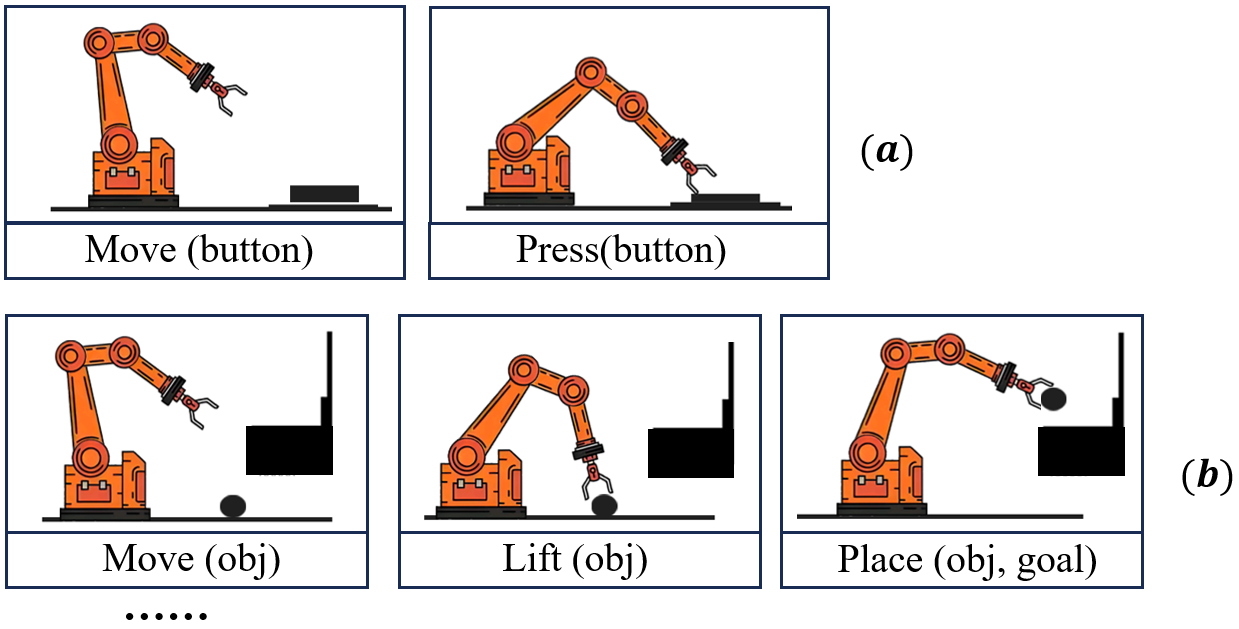
\includegraphics[width=0.48\textwidth]{F-1-1.PNG} 
\caption{Illustration of a robotic arm and its 2 tasks: (\textit{a}) \textsc{Press-Down}, (\textit{b}) \textsc{Pick-and-Put}. The tasks are staged, and there are intercorrelations between the stages from different tasks.}
\label{fig:task_sim}
\end{figure}

%MTRL 背景与应用
%\textcolor{blue}{1. Multi-task reinforcement learning (MTRL) is useful. MTRL Background and Applications}

Multi-task reinforcement learning (MTRL) aims to learn a single policy for multiple tasks by leveraging shared representations and experience~\cite{q2}. 
There are many applications of MTRL in practice~\cite{q60}.
For example, robotic arms have become quite prevalent and sophisticated in modern manufacturing \cite{q45}.
As shown in Fig.~\ref{fig:task_sim}, a robotic arm is often designed to handle multiple operations (e.g., moving, pressing, pushing) on different objects.
Since a robotic arm typically operates under consistent physical conditions and tasks are often interrelated, MTRL offers a practical solution for task execution.
It has been reported that, in such cases, MTRL may effectively enhance data utilization and promote knowledge transfer across tasks~\cite{q7}. 

%现有 MTRL 方法回顾
%\textcolor{blue}{2. Review of existing MTRL methods.}
Numerous MTRL approaches have emerged in recent years.
For example, PopArt \cite{q12} extended single-task RL to MTRL by sharing the entire network backbone and evaluated its effectiveness on the Atari-57 benchmark \cite{q81}.
Soft.M \cite{q51} divided the network into several modules and implemented soft sharing \cite{q32} among them via task-specific parameter updates.
To further granulate network sharing, PaCo \cite{q36} used soft masks to enable combinatorial sharing of task-specific parameters, providing fine-grained control at the parameter level.
D2R~\cite{q75} considered different task difficulty levels and combined network modules via a flexible gating mechanism.

%\textcolor{blue}{3. The core challenges and the need to divide them into stages. Why?}
%核心挑战与阶段划分的必要性

Although effective in certain applications, \emph{most existing MTRL methods overlook the characteristics of tasks}.
Consider the control of robotic arms again, as shown in Fig.~\ref{fig:task_sim}.
It can be seen that tasks therein are \emph{structured}, consisting of clear sequenced subtasks (stages).
For example, \textsc{Pick-and-Put} can be decomposed into 4 consecutive stages: \textsc{Move}, \textsc{Grasp}, \textsc{Move}, and \textsc{Place}, whereas \textsc{Open-Drawer} is 3-staged with \textsc{Move}, \textsc{Grasp}, and \textsc{Move} in order.
There is a substantial resemblance between the elementary stages of different tasks.
While some existing MTRL methods exploit task relationships \cite{q39}, there is little discussion of stages or stage-level knowledge transfer.

%表示&策略：为什么需要考虑这两方面，和阶段划分有什么关系。为什么需要表示(其他人做法，预实验，为什么使用VAE),为什么需要策略(软模块，梯度)
In addition, \emph{most MTRL methods rely on elaborate reward functions to guide the learning, which in turn require a high level of expertise in both application (e.g., robot mechanics) and algorithm design} \cite{q79,q80}.
As opposed to such highly directive reward functions are the so-called \emph{sparse rewards}, which merely signal the final successes of (sub)tasks.
We conducted a set of preliminary experiments, the details of which are presented in Section \textcolor{red}{5.2} (Table~\ref{table:s}), to assess the reliance of major MTRL approaches on reward functions.
The results show a significant (16.9\%-34.9\%) percentage decline in task success rates as the rewards get sparse.
The final task success rates are all below 49.1\%, making those approaches ineffective in practice.

Note that task structures and reward signals are inherently linked.
In real-world applications, many users have sufficient domain knowledge to decompose tasks reasonably.
However, they often lack the specialized expertise required to design highly directive reward signals for RL agents.
Therefore, sparse rewards are a natural byproduct of practical task decomposition.
\emph{A key challenge for MTRL is thus to develop methods that can effectively handle structured tasks with sparse reward signals.}

Recent advances in MTRL have investigated the use of richer prior knowledge.
CARE \cite{q69} used natural language task descriptions to help agents better understand tasks and their relationships.
The task descriptions are encoded into contexts to guide the learning.
LEGION \cite{q84} extends the use of natural language as prior knowledge for few-shot lifelong learning.
While these methods improve learning through prior knowledge and enhanced knowledge transfer, they operate at the task level and lack mechanisms for stage-aware policy adaptation.
To the best of our knowledge, \emph{no prior work has thoroughly explored structured sparse-reward tasks in MTRL}.


To bridge the gap between task structure awareness and the practical limitations imposed by sparse reward signals, we propose Stage-Masked Policy (SMP), a unified framework explicitly designed to model, reuse, and adapt to task-stage structures in MTRL. 
SMP assumes each task can be decomposed into interpretable stages using domain knowledge, providing useful structural priors(Section 3).

% \begin{figure}[htbp]
%    \centering
%         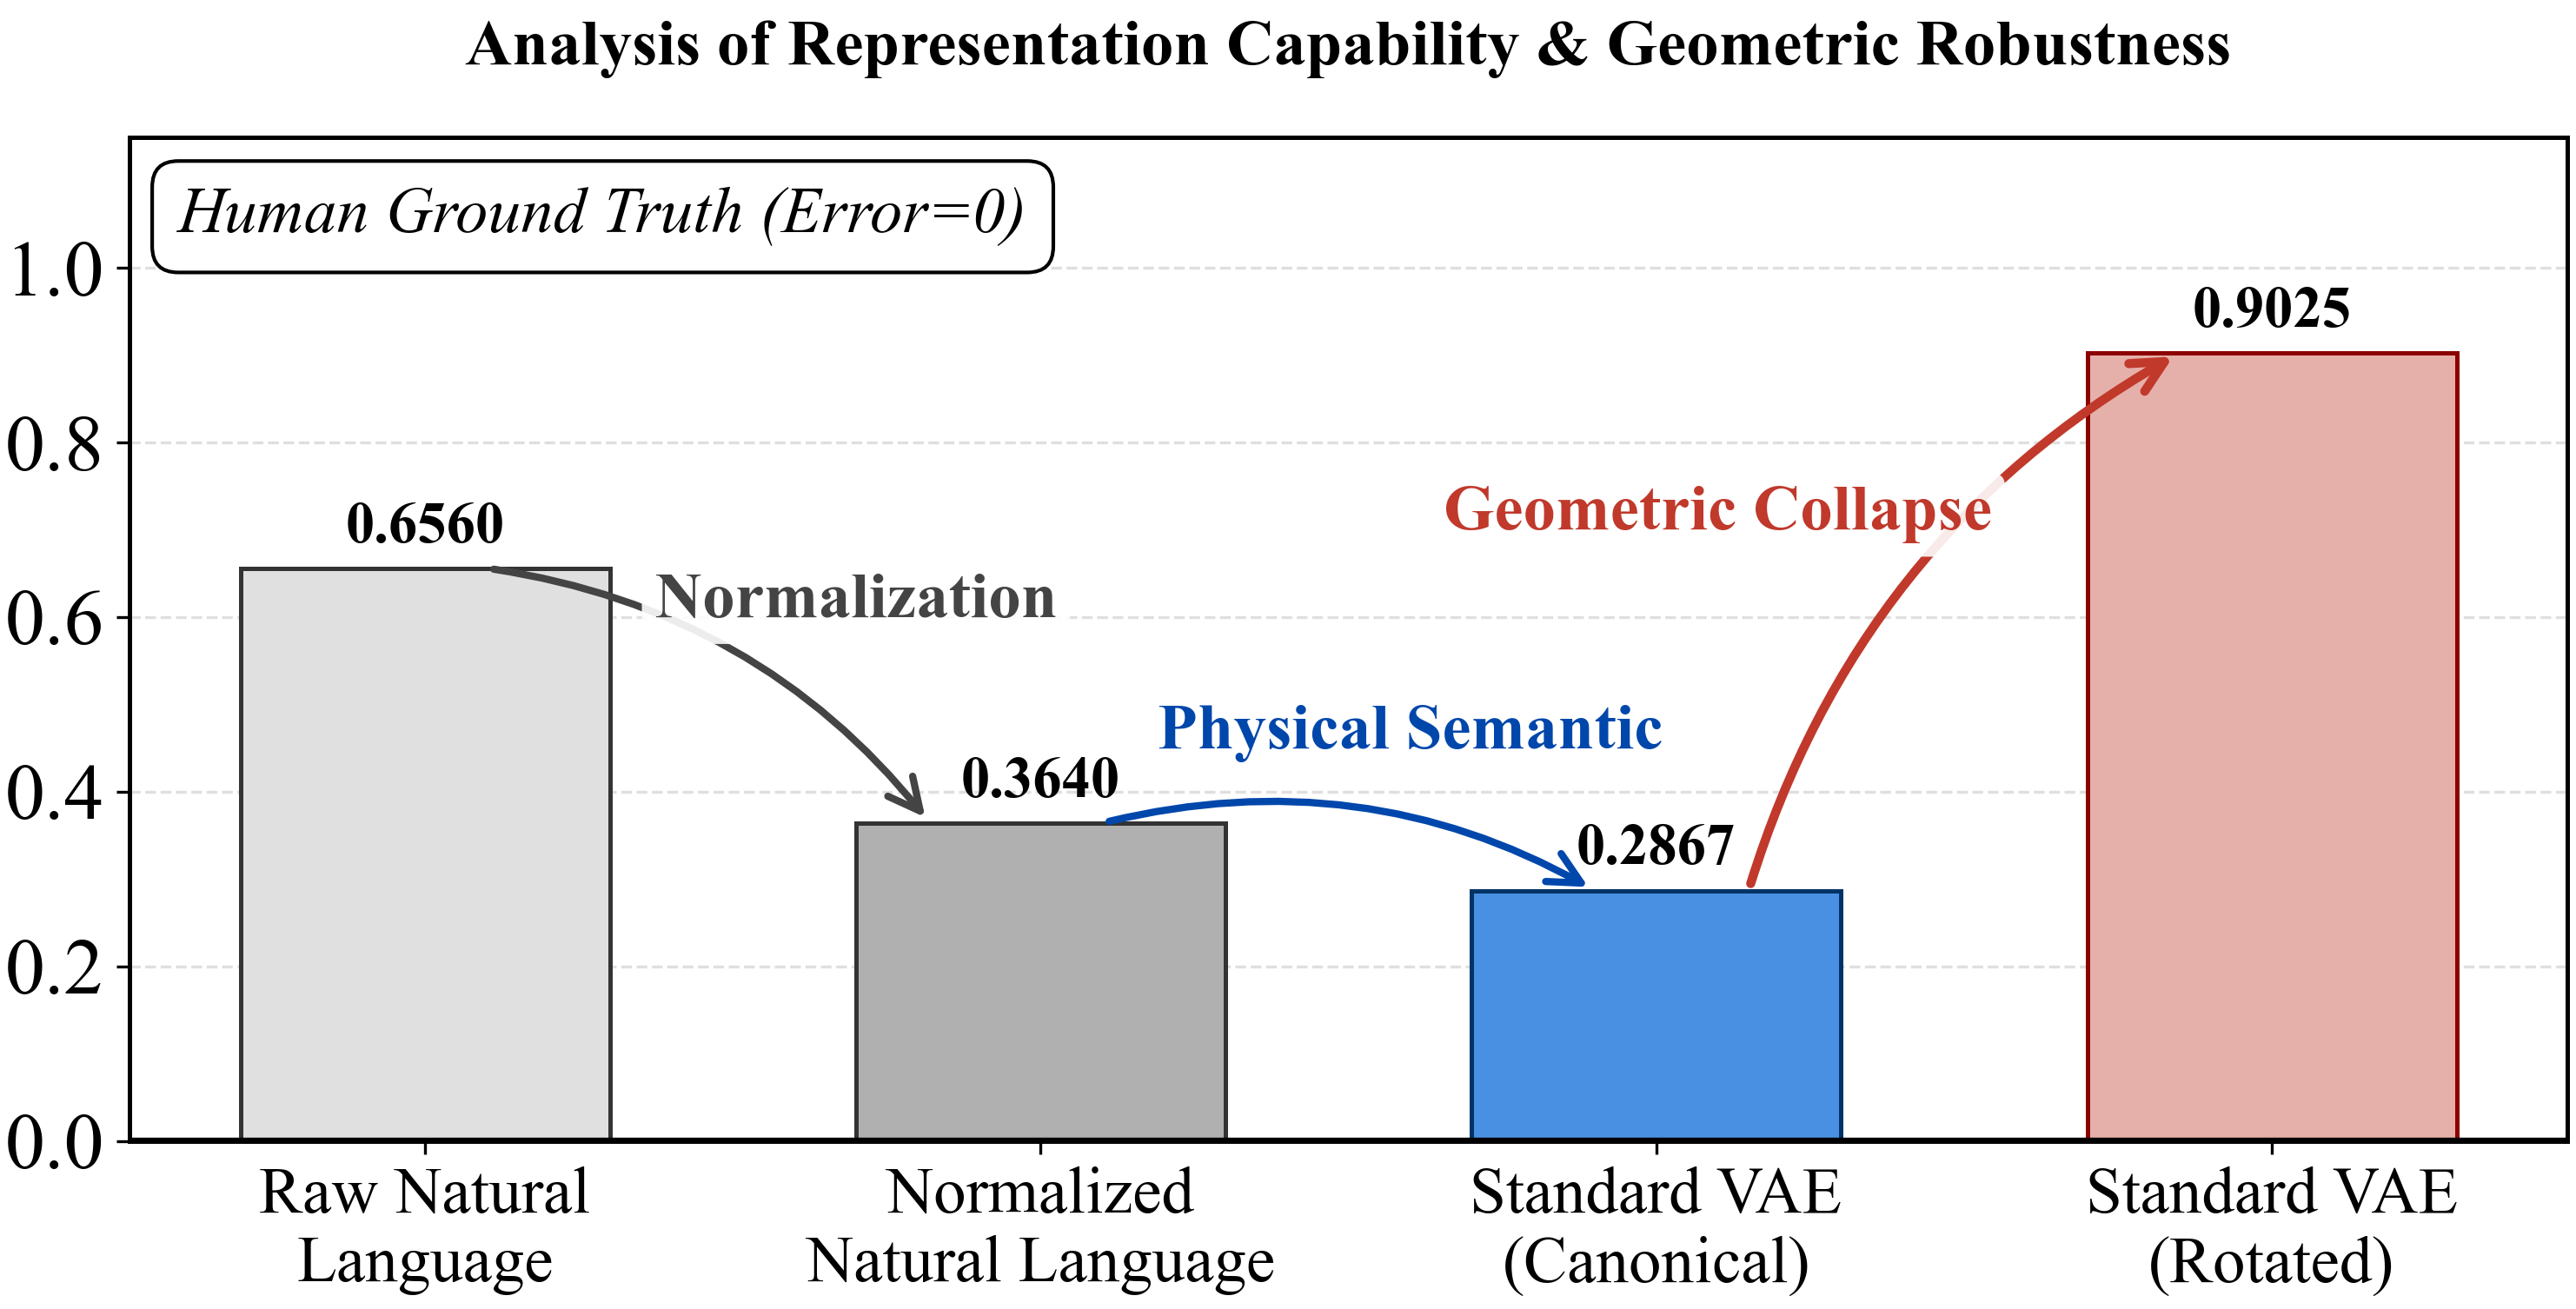
\includegraphics[width=0.48\textwidth]{s-R-6.png} 
% \caption{Statistical comparison of similarity metrics on MT50. Semantic embeddings (Raw: 0.656, Norm: 0.364) show high divergence from human priors. Standard VAEs achieve better alignment (0.287) but fail under geometric rotation (0.903), highlighting the necessity for precise data-driven representations.}
% \label{fig:sim}
% \end{figure}

%1.怎么从上一段先验到问题的；2.为什么需要考虑表示和相似性；3.目前这个相似性能说明什么？4.为什么需要有效几何不变的阶段表示；5.基于相似性和任务差异，我们为什么需要阶段策略来细粒度的学习？
% \textcolor{blue}{
% Although stage decomposition provides a structural skeleton, the fundamental bottleneck remains task heterogeneity. 
% This refers to the diverse physical dynamics across tasks, which create conflicting gradients that hinder unified learning. 
% To address this, we first establish a structural baseline using human priors, defined as binary indicators: 1 for stages executing the same functional predicate and 0 otherwise. 
% However, translating this structure into transferable knowledge requires a precise similarity metric.
% We first benchmarked semantic embeddings derived from BERT. 
% As shown in Fig. ~\ref{fig:sim}, these embeddings significantly diverge from human functional priors (MAE 0.656). 
% This high error empirically proves that linguistic descriptions focus on semantic surface features rather than the underlying kinematic equivalence defined by human experts.
% Consequently, to capture actual physical behaviors, we transition to a data-driven approach using Variational Autoencoders (VAEs) to compress agent trajectories into latent representations. 
% Yet, standard VAEs exhibit a critical flaw: they lack geometric invariance. 
% Under rotational shifts, their recognition error spikes to 0.9025, indicating that they erroneously treat the same physical action as distinct tasks simply due to coordinate changes. 
% This necessitates our use of Geometry-Invariant Representations to accurately align stages regardless of orientation. 
% Finally, accurate representation alone is insufficient because it only identifies heterogeneity without resolving the gradient updates.
% Even with perfect alignment, a shared backbone would still suffer from destructive interference during backpropagation. 
% Therefore, we propose a SMP to explicitly enforce the identified alignments, isolating gradients to compatible subspaces to physically prevent negative transfer.
% }
%回答论证：1.问题: 异质性导致梯度冲突（多任务挑战源泉，也是先验的原因和基础）.   2.确立解决方案的“基线”与“前提”（表示和相似性）  3.这人类先验和自然语言对比，试错，说明需要基于数据和潜在空间表示的VAE.（论证，能说明什么？） 4.VAE还不够，无法处理几何不变。（为什么我们还要做EGNN-VAE？）  5.回到根本，我们还需要结合阶段策略（回归原点&先验&问题），承接下面的贡献

%基于前面的问题，说明解释对应解决方案核心方法
Given these predefined structures, our method focuses on two core modules:
(1) Similarity calculation, which constructs a dynamic similarity matrix from agent trajectories to quantify behavioral alignment between task stages;
(2) Mask-Based Policy Activation, which employs binary masks to selectively activate reusable policies for each stage, enabling stage-level transfer and avoiding negative transfer.
By aligning policy sharing with structural similarities at the stage level, SMP reduces the reliance on carefully engineered reward functions and enables fine-grained, adaptable knowledge transfer.
This approach substantiates our insight: effective MTRL under sparse reward is possible when transfer is conducted at the stage rather than across entire tasks.

%总结创新&贡献
We evaluate SMP on the Meta-World MT10 and MT50 benchmarks \cite{q15}. 
Experiments show that SMP improves convergence speed and final performance, especially in sparse reward scenarios. 
Combined results from few-shot and model-size experiments further indicate its potential for real-world deployment.
Our main contributions are summarized as follows:
\begin{itemize}
\item We systematically demonstrate that stage-level task decomposition is crucial for efficient MTRL, especially under sparse reward conditions.

\item Building upon this structural prior, we propose a novel modular framework featuring stage similarity estimation and mask-based policy activation to enable fine-grained, stage-level knowledge transfer across tasks.

\item  We evaluate SMP across sparse-reward, few-shot, and parameter-constrained setups, consistently surpassing state-of-the-art MTRL baselines.
\end{itemize}





\section{Related Work}
%多任务部分相关工作，分为两个类：1）基于表示，2）基于策略。说明对比我们为什么需要在表示&策略上进行优化
MTRL enables agents to learn a unified model applicable to multiple related tasks by leveraging shared representations and experience ~\cite{q10,q65}. 
Existing approaches can be broadly categorized into representation learning and architecture-based methods. 
Representation learning methods seek to extract effective, shared features to bridge task relationships. 
For instance, CARE~\cite{q69} encodes natural language descriptions into contextual representations, while STARS~\cite{i5} utilizes shared-and-unique feature extractors to foster knowledge synergy. 
Architecture-based methods typically employ a shared network backbone coupled with task-specific modules. 
Soft.M~\cite{q51} adopts a soft modularization mechanism, and PaCo~\cite{q36} uses combinatorial masks for fine-grained parameter sharing. 
PTSL~\cite{q43} introduces projection layers to assign independent network subspaces for each task.
However, most of these approaches operate primarily at the coarse task level. They often rely on global task IDs or raw state statistics, largely overlooking the fine-grained procedural structures. 
This oversight limits their robustness when transferring skills across spatially diverse tasks.

%稀疏奖励相关研究
%阶段划分相关工作，为什么需要阶段划分，为什么需要谓词；结合AAAI稀疏奖励部分’
To address complex long-horizon tasks, recent research has diverged into reward shaping and task decomposition. Regarding rewards, methods like Eureka~\cite{q86} and DrEureka~\cite{q87} utilize Large Language Models (LLMs) to synthesize reward functions from semantic descriptions. 
However, they generally optimize the learning signal while treating the policy as a black box, neglecting explicit architectural alignment. 
Regarding decomposition, approaches utilize linguistic priors~\cite{i9,i8} or latent skill extraction~\cite{i7,i6} to identify interaction phases. 
While these approaches offer practical utility, they face significant challenges: language planning often encounters a “semantic-kinematic gap” related to low-level control, while skill-based methods typically require specifying skill duration or data priors.
Neither effectively enables agents to learn structural from scratch in sparse-reward settings.


%总结&不同，使用在表示层面做了EGNn，在策略层面做了阶段策略掩码
In contrast to these methods, our approach introduces a stage-aware masking framework that activates sub-policies corresponding to interpretable task stages and selectively transfers them across tasks based on quantified stage similarity.
This enables fine-grained knowledge transfer and robust training under sparse reward conditions, which prior approaches often fail to address


\begin{table}[h]
\centering
\resizebox{\columnwidth}{!}{%
\begin{tabular}{@{}lccc@{}}
\toprule
\textbf{Method} & \textbf{Policy Opt.} & \textbf{Rep. Opt.} & \textbf{Granularity} \\
\midrule
MT-SAC \cite{q15}  & $\times$ & $\times$ & Task \\
Soft.M \cite{q51}  & $\checkmark$ & $\times$ & Task \\
CARE \cite{q69}  & $\times$ & $\checkmark$ & Task \\
PaCo \cite{q36}  & $\checkmark$ & $\times$ & Task \\
PTSL \cite{q43}  & $\checkmark$ & $\times$ & Task \\
\textbf{SMP (Ours)}  & $\checkmark$ & $\checkmark$ & \textbf{Stage} \\
\bottomrule
\end{tabular}%
}
\caption{Methods Comparison in Policy, Representation Optimization, and Granularity}
\label{tab:comparison}
\end{table}


\section{Preliminaries}

\paragraph{Structured Tasks \& Stg-MDPs.} We model an $n$-staged task $T$ as a \emph{Staged Markov Decision Process} (Stg-MDP),
\[
T=\left(\mathcal{S},\mathcal{A},\mathcal{P},\mathcal{R},\sigma,H\right),
\]
as illustrated in Fig.\,\ref{fig:mdp}.
Here, $\mathcal{S}=\bigcup_{k=1}^n\mathcal{S}_k$ is the state space, where the subspace $S_k$ is the set of states in the $k$-th stage of the task;
$\mathcal{A}$ is the action space of the agent, as in regular MDPs;
$\mathcal{P}=\bigcup_{k=0}^n\mathcal{P}_k$ is the state transition function, where $\mathcal{P}_k:\mathcal{S}_k\times\mathcal{A}\times\mathcal{S}_k\rightarrow[0,1]$ defines the transition probability within the $k$-th stage ($k>0$) and $\mathcal{P}_0:\mathcal{S}\times\mathcal{A}\times\mathcal{S}\rightarrow[0,1]$ is the probability of rolling back from later stages to previous ones;
$\mathcal{R}=\bigcup_{k=0}^n\mathcal{R}_k$ is the reward function, consisting of the reward functions within each stage, $\mathcal{R}_k:\mathcal{S}_k\times\mathcal{A}\times\mathcal{S}_k\rightarrow\mathbb{R}$, and a penalty function $R_0:\mathcal{S}\times\mathcal{A}\times\mathcal{S}\rightarrow\mathbb{R}$ for stage rolling back;
$\sigma:\mathcal{S}\rightarrow\{1,2,\cdots,n\}$ is the (sub)goal indicator, where $\sigma(s)=k$ indicates $s$ being one of the goal states within the $k$-th stage;
Finally, $H$ is the finite horizon, i.e., the maximum number of steps allowed for an agent to fulfill the task.


\begin{figure}[htbp]
   \centering
        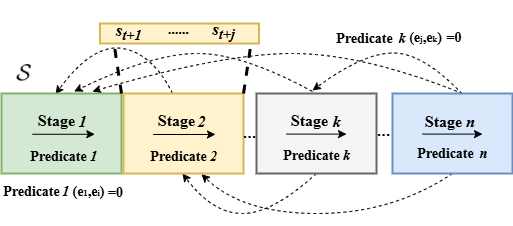
\includegraphics[width=0.48\textwidth]{SMDP-5.png} 
\caption{\hl{Stg-MDP. A Stg-MDP is a sequence of consecutive stages. Each stage is a standard MDP (with its own states, transition function, and reward function), except for possible rolling-back transitions and the corresponding penalties.}}
\label{fig:mdp}
\end{figure}

%问题需要解释：为什么需要预定义的谓词，实体，怎么预定义的。解释谓词和封装好的子过程的区别（任务规划，运动学建模）。
%加入谓词和实体定义，给出谓词&实体作为先验的预定义形式。
To physically instantiate the abstract stage indicator $\sigma$, we augment the MDP with a Symbolic Prior tuple $\langle \mathbb{E}, \mathbb{P} \rangle$.
This formulation grounds the task structure in kinematic data:
\begin{itemize}
\item Entities ($\mathbb{E}$): Let $s \in \mathcal{S}$ be the raw observation vector. 
We define the entity set $\mathbb{E} = \{e_i\}_{i=1}^I$ where each $e_i = \phi_i(s)$ is an explicit sub-vector of $s$ (e.g., end-effector position), derived via observation slicing. 
This ensures the symbolic interface operates on precise physical data.
\item Predicates ($\mathbb{P}$): We define $\mathbb{P} = \{p_j\}_{j=1}^J$ as a set of geometric classifiers $p_j: \mathcal{S} \rightarrow \{0, 1\}$.
These predicates serve as the termination conditions for stages, mathematically formalized as inequalities over entities (e.g., $\texttt{At}(e_1, e_2) \iff \|e_1 - e_2\| \le \delta$).
\end{itemize}

%奖励机-和目前谓词-阶段系统融合
% \paragraph{Predicate-based Reward Machine.}
% To provide dense and structured guidance, we instantiate the reward structure as a Predicate-based Reward Machine\cite{i15}.
% Given the stage decomposition defined by predicates $\mathbb{P}$, we associate each stage $k$ with a specific reward function
% $\mathcal{R}_k: \mathcal{S}_k \times \mathcal{A} \to \mathbb{R}$.
% Each $\mathcal{R}_k$ is mathematically constructed using the relevant entities $\mathbb{E}$ to quantify the progress towards satisfying the current stage's termination condition.
% Functionally, the Reward Machine operates as a dynamic dispatcher.
% At each timestep $t$, it queries the stage indicator $\sigma(s_t)$ derived from the predicate checks.
% Based on the returned stage index, the machine activates the corresponding local reward function to compute the feedback.
% Formally, the reward signal is defined as:
% \begin{equation}
% r_t(s_t, a_t) = \mathcal{R}_{\sigma(s_t)}(s_t, a_t) + \mathbb{I}_{(\text{success})} \cdot r_{\text{success}},
% \end{equation}
% where $\mathcal{R}_{\sigma(s_t)}$ provides the dense shaping signal specific to the active sub-task, and $r_{\text{success}}$ denotes a sparse terminal bonus.This mechanism decomposes the global long-horizon optimization problem into a sequence of simpler, locally guided sub-problems.

% A critical distinction of our setting from Task and Motion Planning (TAMP) is the absence of encapsulated motion primitives.
% While TAMP relies on pre-defined subroutines (e.g., $\texttt{Pick()}$) to execute transitions \cite{i11}, such primitives are often unavailable in contact-rich environments with unmodeled dynamics.
% Therefore, we use predicates $\mathbb{P}$ solely to specify the goal ("What state to reach"), leaving the control execution ("How to reach it") to be autonomously learned by the RL agent.
%实体/谓词的数学定义-物理形式-不同

\paragraph{State representation.} \hl{A state can be represented as a combination of some \emph{predefined} stages.}

\paragraph{Objective.} 
Consider $\mathcal{T} = \{T^{(1)}, T^{(2)}, \dots, T^{(N)}\}$, a set of $N$ structured tasks, where task 
\[
T^{(i)}=\left(\mathcal{S},\mathcal{A},\mathcal{P}^{(i)},\mathcal{R}^{(i)},\sigma^{(i)}, H\right)
\]
with $\mathcal{S}=\bigcup_k\mathcal{S}_k^{(i)}$.
We aim to learn a policy $\pi_{\bm{\theta}}(\cdot | s)$, parameterized by $\bm{\theta}$, that maps a state $s$ to a probability distribution over actions.
The policy $\pi_{\bm{\theta}}$ is to maximize the average expected cumulative return across all tasks in $\mathcal{T}$, i.e.,  
\begin{equation*}
J(\bm{\theta}) = \frac{1}{N} \sum_{i=1}^{N} \mathbb{E}_{\pi_{\bm{\theta}}} \left[ \sum_{t=0}^{H} \mathcal{R}^{(i)}(s_{t}, a_{t}) \right].
\end{equation*}

%\paragraph{Mask-Based Parameter Sharing.} 
%We share a policy parameter across tasks and modulate it via stage-aware masks to achieve adaptive policy behaviors.
%Let $\theta \in \mathbb{R}^d$ denote the parameters of the backbone layer of the policy network $\pi_{\theta}$.
%For each task-stage pair $(i, k)$, we define a binary mask:
%\begin{equation}
%M^{(i)}_{k} \in \{0, 1\}^d,
%\end{equation}
%During task execution, the effective parameters are modulated by the current stage $k$:
%\begin{equation}
%\theta^{(i)}_{k} = \theta \odot M^{(i)}_{k}.
%\label{eq:2}  
%\end{equation}
%Yielding the stage-aware policy:
%\begin{equation}
%\pi^{(i)}(a|s) = \pi_{\theta^{(i)}_{k}}(a|s),
%\end{equation}

%The MTRL objective (Eq.~\ref{eq:2}) is redefined as joint optimization over $\theta$ and mask configurations:
%\begin{equation*}
%\max_{\theta, \{M^{(i)}_{k}\}} 
%J(\theta, \{M^{(i)}_{k}\}) 
%= \frac{1}{N} \sum_{i=1}^{N} 
%\underset{\pi_{\theta^{(i)}_{k}}}{\mathbb{E}}
%\Bigg[ 
%    \sum_{t=0}^{H}
%    \mathcal{R}^{(i)}(s_{t}, a_{t}) 
%\Bigg].
%\end{equation*}

\section{Methodology}

\subsection{Overall Framework}
%不用讲具体方法只讲输入/输出和在整体框架中的作用即可。
\begin{figure*}[!htp]
\centering
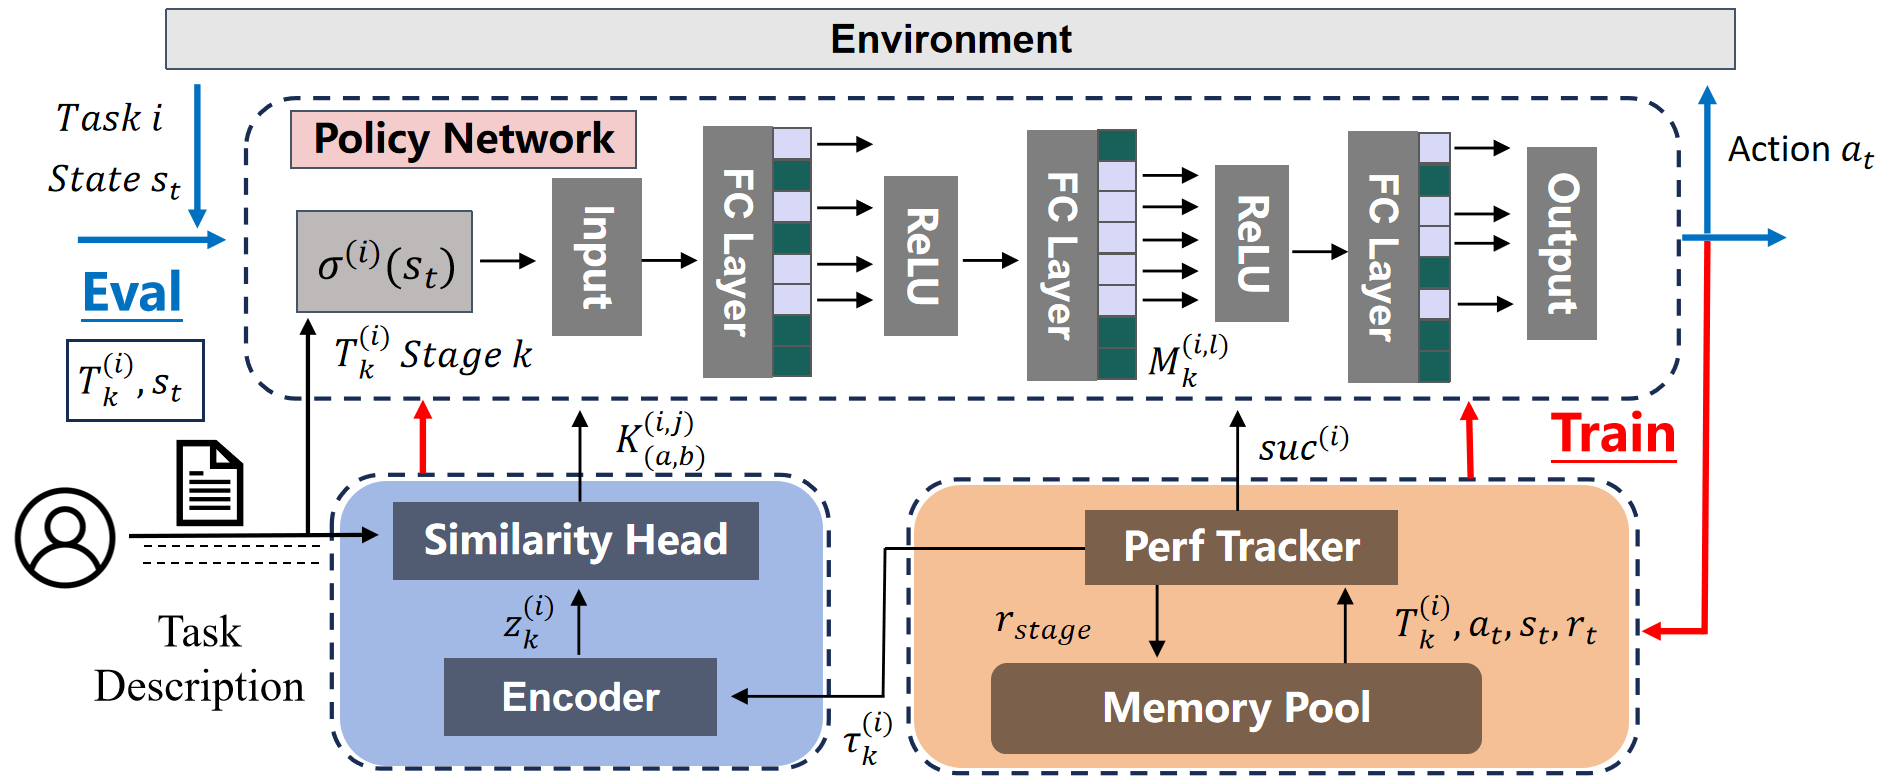
\includegraphics[width=16cm,height=6cm]{F-3.PNG}\\
\caption{
Task states ($s_t$) → Stage Division($\sigma^{(i)}(s_t)$) → Mask-based stage policy ($\pi_{\theta^{(i)}_{k}}(a_t|s_t)$) generate actions ($a_t$). 
}
\label{fig:fig_3}
\end{figure*}

Fig.\,\ref{fig:fig_3} shows our stage-aware MTRL framework named \hl{Stage-Masked Policy (SMP)}.

SMP augments the conventional parameter-sharing paradigm by explicitly modeling the procedural stages of tasks.
It comprises three tightly coupled components that function cyclically to enable fine-grained knowledge transfer:


%阶段划分介绍：输入/输出/作用。
To decompose complex tasks into stages, we employ a deterministic Stage Division Function $\sigma^{(i)}$.
Input/Output: At each timestep $t$, taking the current state $s_t$ and the symbolic priors $\langle \mathbb{E}, \mathbb{P} \rangle$ as input, it outputs a discrete semantic stage index $k_t$:
\begin{equation}
k_t = \sigma^{(i)}(s_t; \mathbb{E}, \mathbb{P}).
\label{eq:stage_division}
\end{equation}
Role: This module acts as a real-time gating mechanism, explicitly explicitly informing the agent of the current execution phase ($k_t$) to trigger the corresponding policy mask.
%阶段划分-输入输出-功能（框架）

%编码器&相似性计算介绍：输入/输出/作用
To determine what knowledge to share across tasks, this module quantifies the kinematic equivalence between stages.
Input/Output: It takes stage-wise trajectories $\tau_k^{(i)}$ as input, encodes them into geometry-invariant latent distributions $z_k^{(i)}$ via an encoder $E_\phi$, and computes a similarity matrix $\mathcal{K}$:
\begin{equation}
\mathcal{K}{(a,b)}^{(i,j)} = \text{SIM}(z_a^{(i)} | z_b^{(j)}), \quad \text{where } z \leftarrow E_{\phi}(\tau).
\label{eq:similarity}
\end{equation}
Role: The matrix $\mathcal{K}$ serves as a transfer map, guiding the policy to inherit parameters from physically similar stages (high similarity).
%数据输入-编码器（潜变量）-相似性-指导策略

%最重要的阶段掩码策略：输入/输出/作用
Finally, the agent executes actions using a shared backbone modulated by topological masks.
Input/Output: Conditioned on the stage index $k$ and the similarity guidance $\mathcal{K}$, the policy activates a specific binary mask $M_{k}^{(i)}$. The action $a_t$ is generated by the masked parameters:
\begin{equation}
a_t \sim \pi_{\theta}(a_t | s_t; \theta \odot M_{k}^{(i)}).
\label{eq:policy_execution}
\end{equation}
Role: This mechanism enforces strict gradient isolation by physically blocking interference between unrelated stages, ensuring that parameter updates are confined to the relevant functional sub-network.

\subsection{Predicate-based Structured Stage Division}


\renewcommand{\algorithmicrequire}{\textbf{Input:}}
\renewcommand{\algorithmicensure}{\textbf{Output:}}
\begin{algorithm}[t]
\caption{Predicate-based Stage Identification}
\label{alg:stage_id}
\begin{algorithmic}[1]
\REQUIRE Current State $s_t$, Entity Set $\mathbb{E}$, Conditions $\{\mathcal{C}_k\}_{k=1}^n$ derived from $\mathbb{P}$
\ENSURE Active Stage Index $k_t$

\FOR{$k = 1$ \textbf{to} $n$}
    \STATE \textbf{if} $\mathcal{C}_k(s_t; \mathbb{E}) = 0$ \textbf{then return} $k$
\ENDFOR

\RETURN $n + 1$ 
\end{algorithmic}
\end{algorithm}


%在这里只讲“怎么用”，结合 Algorithm 1，重点描述运行时的逻辑
Given the symbolic priors defined in Section 3, we implement the stage division function $\sigma^{(i)}$ as a deterministic, real-time gating mechanism.
Its primary role is to dynamically map the continuous state stream $s_t$ into a discrete stage index $k_t$, which subsequently triggers the stage-specific encoder and policy modules.

As formalized in Algorithm~\ref{alg:stage_id}, the function $\sigma^{(i)}$ evaluates the task progress at each timestep.
Our module operates online by checking the sequence of stage conditions $\{\mathcal{C}_k\}_{k=1}^n$ derived from $\mathbb{P}$.
Specifically, the logical flow follows a waterfall mechanism:
\begin{equation}
k_t = \min\{ k \mid \mathcal{C}_k(s_t; \mathbb{E}) = 0 \}
\end{equation}
The agent is considered to be in stage $k$ if all preceding conditions $\mathcal{C}_{1 \dots k-1}$ are satisfied, but $\mathcal{C}_k$ is not.
This sequential evaluation ensures that the agent strictly follows the procedural hierarchy of the task.
By continuously monitoring the geometric relations between entities , it provides stable structural indices.
%为了利用任务结构先验，我们使用前面提到的谓词逻辑来阶段划分。




\subsection{Encoder and Similarity Calculation}

%解释为什么光有谓词不够，必须要有基于数据的表示。结合Intro,衔接上面的工作，确保逻辑通顺。（提出问题，回答问题）
\paragraph{Motivation.}
While the predicate-based division (Section 4.2) provides discrete structural indices, it does not quantify the kinematic heterogeneity across tasks.
As demonstrated in our Introduction (Figure 2), merely sharing parameters based on semantic labels is insufficient due to diverse physical dynamics and geometric shifts.
Therefore, effective transfer requires a representation that is both functionally distinct and geometrically invariant.
%逻辑链：结构有了-但物理细节缺失-且存在几何干扰-需要新表示。

%基于数据，基于什么数据？定义输入数据。高奖励序列
We adopt a data-driven approach to capture stage-specific dynamics.
Using the indices $k_t$ from the Stage Division Function, we define a Stage Trajectory $\tau^{(i)}_{k}$ as a sequence of state-action pairs $\{(s_t, a_t)\}_{t=1}^{L}$.
To ensure the representation encodes optimal behaviors rather than exploration noise, we maintain a prioritized buffer that stores only high-return trajectories satisfying a length threshold $L_{\min}$.
%逻辑链：为了学表示 - 收集高分轨迹-输入进 EGNN-CVAE 模型。同时能详细解释这个模块的输入

\begin{figure}[htbp]
   \centering
        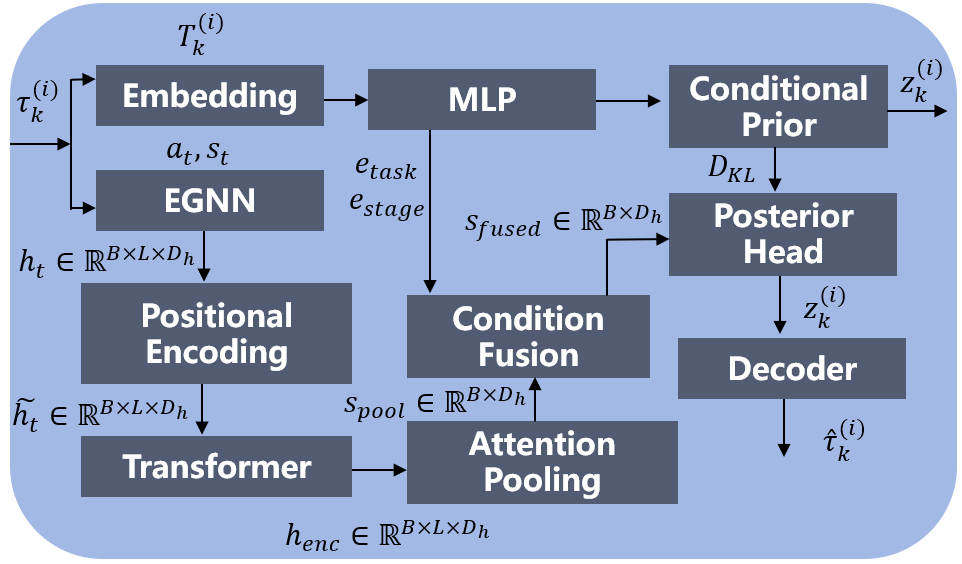
\includegraphics[width=0.48\textwidth]{E-2.png} 
\caption{Architecture of the EGNN-CVAE Encoder. It utilizes an SE(3)-invariant graph frontend to extract geometric features, followed by a Transformer for temporal aggregation, producing a latent distribution $z$ robust to spatial transformations.}
\label{fig:encoder}
\end{figure}


%怎么利用数据。介绍创新部分；给出框架&创新。%怎么利用数据。
\paragraph{Conditioned SE(3)-Invariant Frontend.}
A key challenge in trajectory modeling is the misalignment between spatial geometry and semantic intent. 
Conventional encoders often lack $SE(3)$-invariance, meaning they perceive the same physical action as distinct tasks when subjected to rotations or translations. 
To overcome this. As shown in Figure~\ref{fig:encoder}, we design a Conditioned SE(3) Frontend that integrates EGNN-based message passing with gating. 
At each time step $t$, the module constructs a fully connected graph among entities (e.g., hand, object, goal) and updates node embeddings using relative coordinates, ensuring global frame invariance:
\begin{equation*}
\mathbf{h}_t = \mathrm{EGNN}(s_t, a_t).
\end{equation*}


We add sinusoidal positional encodings to preserve temporal order:
\begin{equation*}
\tilde{\mathbf{h}}_t = \mathrm{PE}(\mathbf{h}_t).
\end{equation*}

%方法流程，方法&组件流水账，但是必须讲解清晰，不能随便给出新的定义
\paragraph{Encoder $E_{\phi}$ Pipeline.}
The encoder comprises three stages capturing both spatial and temporal dependencies:

\begin{enumerate}
    \item Invariant Feature Extraction: The SE(3) Frontend outputs geometry-invariant node features $\mathbf{h}_t$, enhanced with positional encodings $\tilde{\mathbf{h}}_t$ to retain temporal structure.
    
    \item Temporal Aggregation: A multi-layer Transformer encoder processes $\tilde{\mathbf{h}}_{1:L}$ to capture long-range spatiotemporal correlations. 
    An attention pooling layer aggregates the sequence into a global stage descriptor:
    \begin{equation*}
    \mathbf{s}_{\mathrm{pool}} = \mathrm{AttnPool}\!\left(\mathrm{Transformer}\!\left([\tilde{\mathbf{h}}_1, \ldots, \tilde{\mathbf{h}}_L]\right)\right).
    \end{equation*}

    \item Enhanced Conditional Projection: To fuse trajectory semantics with contextual information, we employ an Enhanced Residual Gated Block instead of simple concatenation. 
    Given the condition vector $\mathbf{c}$ (the concatenation of task and stage embeddings), we compute:
    \begin{equation*}
    \mu, \log\sigma^2 = \mathrm{MLP}\!\left(\mathrm{LayerNorm}\!\big(\mathbf{s}_{\mathrm{pool}} + \mathrm{GLU}(\mathbf{s}_{\mathrm{pool}}, \mathbf{c})\big)\right),
    \end{equation*}
    which parameterizes the posterior $q(z \mid \tau, \mathbf{c})$. 
    The corresponding conditional prior $p(z \mid \mathbf{c})$ represents the ideal behavior distribution inferred solely from task attributes.
\end{enumerate}

%讲解在这个模块下，阶段特征怎么得到的：VAE机制
We define the latent stage feature as the mean of the conditional prior:
\begin{equation*}
z^{(i)}_{k} \triangleq \mu^{(i)}_{k,p}, \quad p^{(i)}_{k}(z) = \mathcal{N}\!\left(z \mid \mu^{(i)}_{k,p}, \sigma^{2 (i)}_{k,p}\right).
\end{equation*}
The feature $z^{(i)}_{k}$ captures semantic and geometry-invariant information for stage $(i,k)$ and is concatenated with the state $s_t$ to guide the policy network.

%相似性的计算
\paragraph{Similarity Computation.}
The similarity between two stages $(i,a)$ and $(j,b)$ is determined by comparing their learned priors $p^{(i)}_{a}(z)$ and $p^{(j)}_{b}(z)$, denoted $P_a$ and $P_b$. 
We employ the J-divergence between diagonal Gaussians to measure distributional overlap:
%\begin{equation*}
%D_{J}(P_a \,\|\, P_b) = \tfrac{1}{2}\!\left(D_{KL}(P_a \,\|\, P_b) + D_{KL}(P_b \,\|\, P_a)\right).
%\end{equation*}
The normalized similarity matrix $\mathcal{K}$ is constructed as:
\begin{equation}
\mathcal{K}^{(i,j)}_{(a,b)} = 1 - \frac{D_{J}(P_a \,\|\, P_b) - D_{J}^{\min}}{D_{J}^{\max} - D_{J}^{\min}},
\end{equation}
mapping divergence values to $[0,1]$. 
Larger $\mathcal{K}$ implies higher semantic equivalence and thus stronger parameter sharing during policy optimization.

%整体模块训练逻辑&目标
\paragraph{Hybrid Training Objective.}
The encoder is trained end-to-end by maximizing a hybrid Evidence Lower Bound  objective, integrating reconstruction fidelity, latent regularization, and semantic discriminability:
\begin{equation}
\mathcal{L} = \mathcal{L}_{\mathrm{recon}} + \beta \cdot \mathcal{L}_{\mathrm{KL}} + \lambda \cdot \mathcal{L}_{\mathrm{cls}}.
\end{equation}
Here:
\begin{itemize}
    \item $\mathcal{L}_{\mathrm{recon}} = \mathbb{E}_{q(z|\tau, \mathbf{c})}[\|\hat{\tau} - \tau\|^2]$ reconstructs trajectory sequences,
    \item $\mathcal{L}_{\mathrm{KL}} = D_{KL}(q(z|\tau,\mathbf{c})\,\|\,p(z|\mathbf{c}))$ enforces latent regularity (with a Free Bits constraint to prevent posterior collapse),
    \item $\mathcal{L}_{\mathrm{cls}}$ is an auxiliary cross-entropy classification loss ensuring the latent mean $\mu$ remains predictive of the ground-truth task-stage identity.
\end{itemize}

This hybrid loss jointly enforces geometry invariance, semantic clustering, and discriminative alignment, ensuring that the latent space encodes transferable procedural knowledge across diverse tasks.


\subsection{Stage-aware Masked Policy}

%核心动机，给出使用掩码的理论分析和支撑
\paragraph{Motivation.}

Formally, MTRL aims to optimize a shared parameter vector $\theta \in \mathbb{R}^D$ to minimize the average loss 
$\mathcal{L}(\theta) = \frac{1}{N}\sum_{i=1}^N \mathcal{L}_i(\theta)$ across $N$ tasks.
However, the optimization landscape is plagued by gradient conflict, defined as the negative cosine similarity between gradients of distinct tasks ($\langle \mathbf{g}_i, \mathbf{g}_j \rangle < 0$).
Existing gradient projection methods address this by projecting a task gradient $\mathbf{g}_i$ onto the normal plane of conflicting gradients, resulting in a modified update vector $\mathbf{d}_{proj}$ \cite{i12,i14}.
While this mitigates interference, we argue it represents a optimization-level compromise.


Drawing from the convergence analysis in CAGrad \cite{i12}, the convergence rate of multi-task descent at iteration $t$ is theoretically bounded by the norm of the update direction $\mathbf{d}_t$:
\begin{equation}
\min_{0 \le t \le T} \mathbb{E}\left[ |\nabla \mathcal{L}(\theta_t)|^2 \right] \le \mathcal{O}\left( \frac{1}{\sqrt{T}} \cdot \frac{1}{|\mathbf{d}_t|} \right)
\label{eq:convergence_bound}
\end{equation}
Crucially, projection operations inherently satisfy 
$|\mathbf{d}_{proj}| < |\mathbf{g}_{orig}|$, where $\mathbf{g}_{orig}$ represents the unbiased aggregate gradient. 
This Gradient Norm Reduction implies that resolving conflict via projection shrinks the update step in conflict regions, theoretically slowing down convergence or biasing the trajectory towards sub-optimal Pareto stationary points where gradients vanish due to cancellation rather than optimality.

%定义问题（梯度冲突）-现有解法（为什么使用掩码）-提出方案-理论支撑 


%讲解掩码的定义和作用，呼应上面的理论分析。1.引出 SMP 作为拓扑层面的解决方案。2.定义掩码是如何加在网络上的.3.基于刚才的定义，我们怎么解决梯度冲突的？（屏蔽而不是投影）4.证明 SMP 通过消除重叠项，既解决了冲突，又保留了梯度模长（解释为什么用这个方法）
\paragraph{Masking Mechanism: Design and Rationale}

To avoid this gradient norm reduction trap, we propose a Topological Solution via Stage-Aware Masking.
Instead of modifying the gradient vector itself, we modify the network topology to physically isolate conflicting gradients.
We designate a set of fully connected layers as masked layers $\mathbb{L}_{mask}$ and instantiate a learnable mask vector $M^{(i)}_{k} \in \mathbb{R}^{D_l}$ for each stage $k$ of task $i$.
Formally, the forward propagation for a layer $l \in \mathbb{L}_{mask}$ is modulated as:
\begin{equation}
\mathbf{h}^{(l)}_{out} = (\mathbf{W}^{(l)} \cdot \mathbf{h}^{(l)}_{in}) \odot \sigma(M^{(i,l)}_{k}),
\label{eq:mask_def}
\end{equation}
where $\odot$ denotes the Hadamard product, and $\sigma(\cdot)$ is the sigmoid function relaxed for differentiability.

Based on this definition, the interference term for a specific parameter dimension $d$ is reformulated as:
\begin{equation}
\mathcal{I}_d(\theta) = \underbrace{(\sigma(m_d^{(i)}) \cdot \sigma(m_d^{(j)}))}_{\text{Topology Overlap}} \cdot \underbrace{\langle \nabla_{\theta_d}\mathcal{L}^{(i)}, \nabla_{\theta_d}\mathcal{L}^{(j)} \rangle}_{\text{Gradient Conflict}}.
\label{eq:interference}
\end{equation}
Here, $m_d$ denotes the $d$-th element of the mask vector $M$.
Unlike projection methods that manipulate the Gradient Conflict, SMP employs sparsity regularization to drive the Topology Overlap towards zero for conflicting dimensions.
This achieves Asymptotic Gradient Isolation: it eliminates interference $\mathcal{I}_d \to 0$ without altering the gradient magnitude within the active subspace (i.e., $\| \sigma(m^{(i)}) \odot \mathbf{g}_i \| \approx \| \mathbf{g}_i \|$).
Consequently, each task optimizes at full velocity within its orthogonal subspace, theoretically preserving the convergence properties of single-task learning.
%逻辑链条：掩码定义-作用机制-结合理论-最终结论

%掩码机制怎么更新的，给出具体流程，方法说明和解释
\paragraph{Structural Self-Evolution: Pruning and Regrowth} To automatically discover optimal sub-network topologies without manual engineering, we introduce a continuous Structural Evolution process driven by synaptic importance.

Synaptic Importance Estimation:
We define the importance $\mathcal{I}^{(l)}_{u}$ of neuron $u$ by fusing its weight magnitude and dynamic gradient sensitivity:
\begin{equation}
\mathcal{I}^{(l)}_{u} = |w^{(l)}_{u}| \cdot \left(1 + \frac{|\nabla_{w} \mathcal{L}|}{\mathbb{E}[|\nabla \mathcal{L}|] + \epsilon}\right).
\end{equation}
High gradient sensitivity prevents the premature pruning of low-magnitude but active weights.

Adaptive Pruning and Regrowth:
We construct a binary target mask $T$ by retaining the top-$\rho$ percent of neurons based on $\mathcal{I}$. 
The mask parameters $M$ are optimized to match $T$ via a Binary Cross-Entropy loss. Crucially, the sparsity ratio $\rho$ is adaptive to the task success rate $suc^{(i)}$:
\begin{equation}
\rho(suc^{(i)}) = \rho_{\text{min}} + (\rho_{\text{max}} - \rho_{\text{min}}) \cdot (1 - suc^{(i)}).
\end{equation}
This creates a feedback loop: low-performing stages utilize dense networks ($\rho \to \rho_{\text{max}}$) for exploration, while high-performing stages automatically sparsify ($\rho \to \rho_{\text{min}}$) to lock onto minimal effective structures.
To prevent topological stagnation, we implement Stochastic Regrowth: when performance plateaus at a low level, we randomly reactivate zero-masked connections with probability $p_{\text{regrow}}$, reintroducing plasticity.

%怎么基于相似性进行迁移的，迁移学习
\paragraph{Similarity-Guided Structural Transfer}
While local evolution optimizes topology based on gradient signals, it lacks cross-task insight. We leverage the semantic similarity matrix $\mathcal{K}$ to facilitate Structural Distillation.
During evaluation, a low-performing stage $(j, b)$ can inherit structural priors from a high-performing stage $(i, a)$.
The student's mask is updated via stochastic interpolation:
\begin{equation}
M^{(j,l)}_{b} \leftarrow \mathcal{B} \cdot M^{(i,l)}_{a} + (1 - \mathcal{B}) \cdot M^{(j,l)}_{b},
\end{equation}
where $\mathcal{B} \sim \text{Bernoulli}(\eta \cdot \mathcal{K}^{(i,j)}{(a,b)})$ is a binary sampling variable and $\eta$ is the transfer strength.
By directly copying effective neural pathways from semantically similar stages, this mechanism provides the student with a "winning lottery ticket" learning, accelerating convergence in settings.


\section{Experiment}

\subsection{Experiment Setting}

We evaluate our framework on the widely used Meta-World \cite{q15} benchmark, specifically the MT-10 and MT-50 multi-task suites. 
To assess robustness under varying supervision levels, we conduct experiments in both standard dense-reward settings and challenging sparse-reward scenarios. 
These environments feature diverse robotic manipulation tasks (e.g., reaching, grasping, placing) with inherent sequential structures, making them ideal testbeds for stage-aware policy learning.

All methods are trained for 1 million environment steps to balance efficiency and convergence. 
Metrics are reported using smoothed success rates to reflect stable performance. 
Results are averaged over four random seeds for dense settings and three seeds for sparse settings to ensure statistical reliability. 
To empirically justify our stage-wise modeling, we also provide a detailed analysis of behavioral similarity matrices in Appendix~A, demonstrating that stage-level correlations exhibit richer structures than task-level baselines.


\textbf{Baselines:} We compare SMP with five representative methods:
(i) \textbf{MT-SAC} \cite{q15}: An extension of Soft Actor-Critic for multi-task settings, representing the hard parameter sharing baseline.
(ii) \textbf{Soft.M} \cite{q51}: Employs a soft routing mechanism to dynamically compose shared modules across tasks.
(iii) \textbf{CARE} \cite{q69}: Enhancing task representation learning through task natural language description.
(iv) \textbf{PTSL} \cite{q43}: Based on the shared backbone strategy, a task-specific projection layer is introduced for each task.
(v)  \textbf{PaCo} \cite{q36}: Combines task-specific parameters via parameter recombination weighted by learned coefficients.




\subsection{Experimental Results}

\paragraph{Performance Comparison.}


Based on the experimental setup described above, we comprehensively compare SMP with all baselines in terms of average success rate, convergence speed, parameter efficiency, and training stability.

\begin{figure*}[htp]
\centering
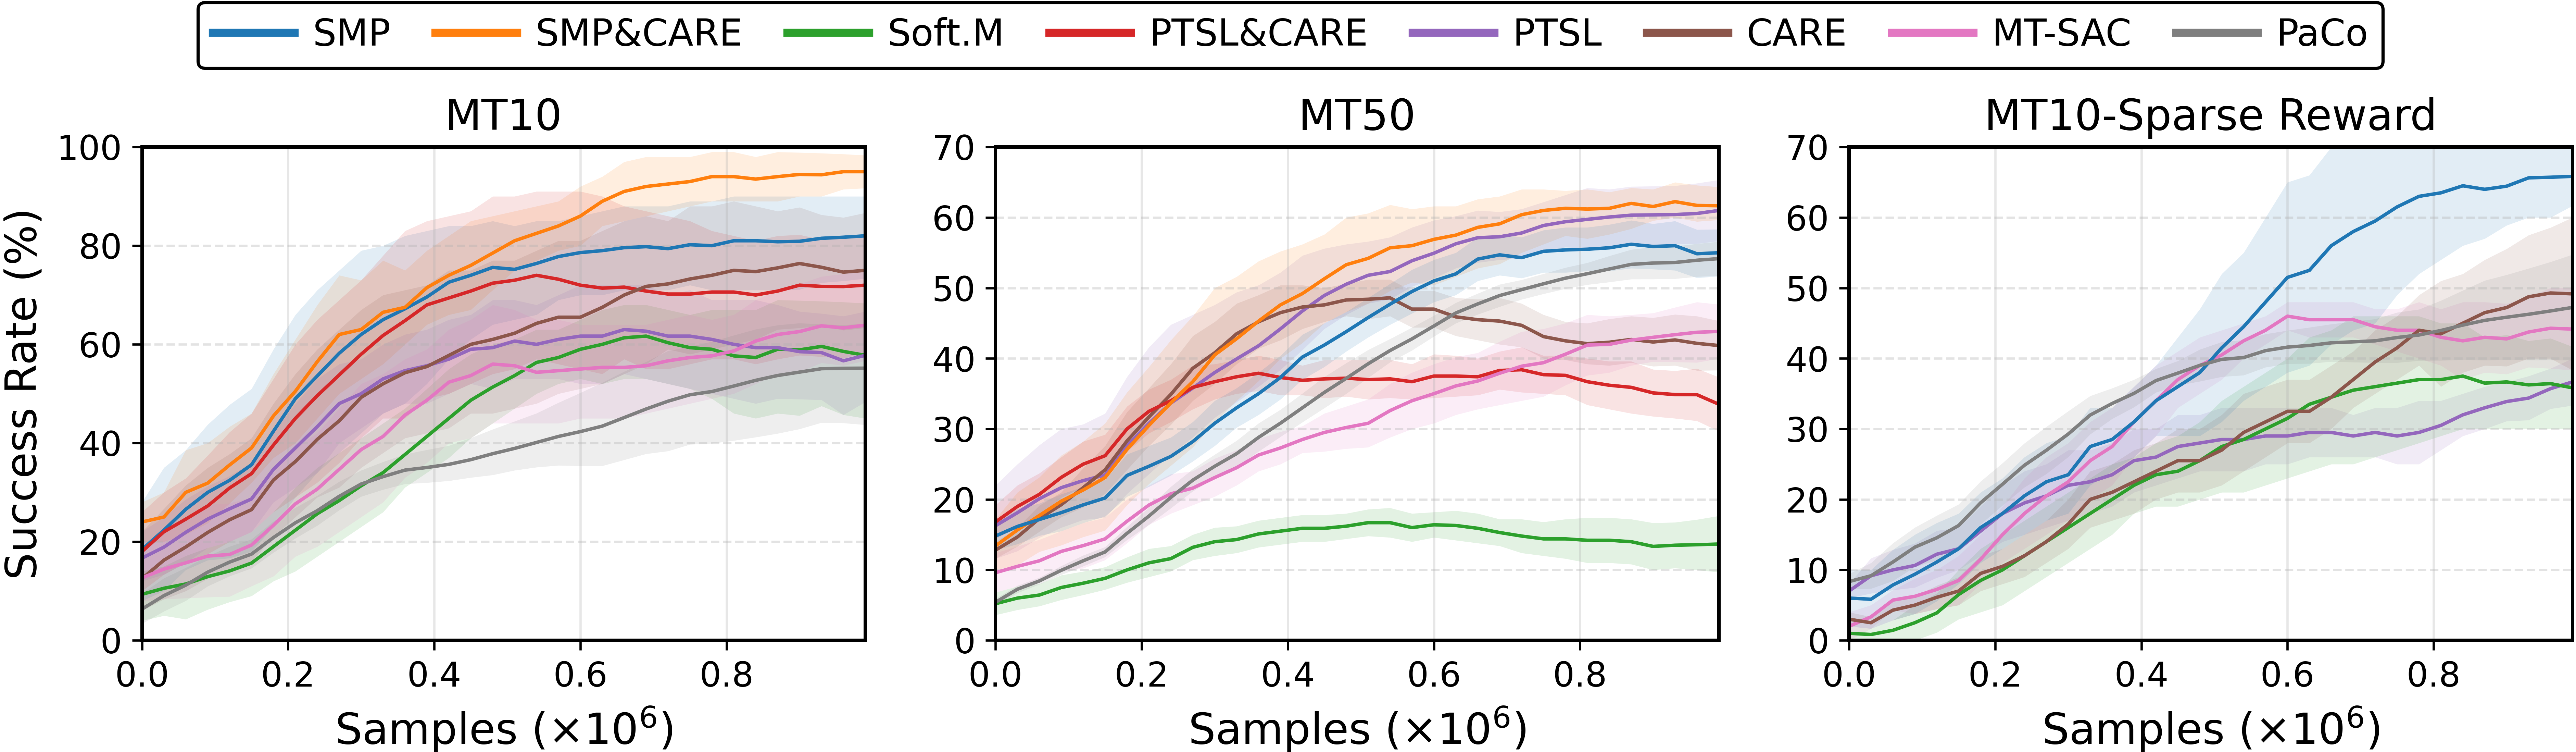
\includegraphics[width=14.4cm,height=4cm]{L-8.png}\\
\caption{Comparison of SMP against baselines on one benchmark setting.}
\label{fig:fig_l}
\end{figure*}

As illustrated in Fig.~\ref{fig:fig_l}, SMP consistently achieves the highest average success rate and the fastest convergence across all evaluated methods. We attribute this performance gain to the stage-aware modular design, which enables efficient knowledge reuse and reduces negative interference between task stages.

For a fair comparison, all models are implemented with comparable network architectures and hyperparameters (Appendix~B). 
Table~\ref{table:m} reports the success rates under three model sizes. Notably, when combined with CARE, SMP achieves a peak accuracy of 95.0\%. 
These results demonstrate both the compactness and the compositional synergy enabled by our approach.

We further assess training stability. 
As shown in Table~\ref{table:s}, SMP yields the lowest standard deviation and highest minimum score, indicating robust convergence. 
This improvement is mainly attributed to mask-based stage policy activation, which effectively reduces interference between tasks and leads to more stable training.



\begin{table}[htbp]
  \centering
  \begin{tabular}{c cc ccc}
    \toprule
    \multirow{2}{*}{\textbf{Methods}} & 
    \multicolumn{2}{c}{\textbf{MT-10(\%)}} & 
    \multicolumn{2}{c}{\textbf{MT-50(\%)}} \\
    \cmidrule(lr){2-3} \cmidrule(lr){4-5}
    &  \textbf{Mean} & \textbf{SD} & 
     \textbf{Mean} & \textbf{SD} \\
    \midrule
    MT-SAC          & 44.1 & -  & 35.0 & - \\
    Soft.M          & 35.8  & -  & 13.1  & -   \\
    CARE            & 49.1  & -  & 20.6 & - \\
    PTSL            & 36.6  & -  & 27.6  & -   \\
    PTSL\&CARE      & 56.6  & -  & 35.3  & - \\
    PaCo            & 47.2  & -    & 7.6   & -   \\
    \midrule
    \textbf{SMP (Ours)}     & \textbf{62.5} & - & \textbf{39.5}  & -  \\
    \textbf{SMP\&CARE}       & - & - & -  & - \\
    \bottomrule
  \end{tabular}
    \caption{Success rate (\%) comparison on MT-10 and MT-50 with \textbf{Sparse} rewards.}
      \label{table:s}
\end{table}

\begin{table}[htbp]
  \centering
  \begin{tabular}{c cc ccc}
    \toprule
    \multirow{2}{*}{\textbf{Methods}} & 
    \multicolumn{2}{c}{\textbf{MT-10(\%)}} & 
    \multicolumn{2}{c}{\textbf{MT-50(\%)}} \\
    \cmidrule(lr){2-3} \cmidrule(lr){4-5}
    &  \textbf{Mean} & \textbf{SD} & 
     \textbf{Mean} & \textbf{SD} \\
    \midrule
    MT-SAC          & 63.8 & 4.7  & 43.4 & 2.5 \\
    Soft.M          & 53.8  & 9.0  & 13.6  & 4.0   \\
    CARE            & 77.0  & 7.1  & 45.3 & 2.8 \\
    PTSL            & 60.4 & 6.1  & 61.6  & 6.6   \\
    PTSL\&CARE      & 74.4  & 4.1  & 33.4  & 3.1 \\
    PaCo            & 56.8  & 10.1    & 54.4   & 5.7   \\
    \midrule
    \textbf{SMP (Ours)}     & \textbf{81.2} & \textbf{3.2} & 55.0  & \textbf{2.1}  \\
    \textbf{SMP\&CARE}       & \textbf{93.3} & \textbf{1.6} & \textbf{62.2}  & 7.7 \\
    \bottomrule
  \end{tabular}
    \caption{Success rate (\%) comparison on MT-10 and MT-50 with \textbf{Dense} rewards.}
      \label{table:d}
\end{table}



We further evaluate SMP’s few-shot adaptability scenarios; results and analysis are detailed in Appendix.B

\paragraph{Sparse Reward.}

To assess robustness under minimal supervision, we evaluate all methods in a sparse reward setting, where agents receive $r = -1$ at every step unless a task is completed ($\sigma^{(i)}_{n}(s)=1$). This simulates realistic scenarios where dense reward is unavailable.


As shown in Table~\ref{table:s}, most baselines perform poorly due to vanishing gradients and insufficient exploration. 
In contrast, SMP achieves a $62.5\%$ success rate, significantly higher than all baselines. 
We attribute this improvement to two key mechanisms in our framework: (1) the stage reward, which provides intermediate intrinsic feedback at stage transitions, thereby alleviating sparse supervision and improving credit assignment; and (2) the stage-masked policy, which enables finer-grained action control through stage-specific policies.
These mechanisms work in concert to enable stable and efficient learning in sparse-reward multitask settings. We further analyze their individual and combined contributions through targeted ablation studies in Section~5.3.





\subsection{Ablation Studies}

First, we perform an ablation experiment on the frequency parameter $B$ governing the use of SMP. 
In our design, the evaluation interval $B$ governs multiple functionalities simultaneously: (1) the mask update and pruning/regrowth cycles, (2) cross-stage similarity calculation, and (3) obtaining high-return action subsequences within a certain interval.  
Table~\ref{tab:eval_interval} reports performance under different evaluation intervals. 

The results clearly indicate that reducing the usage frequency of SMP leads to a degradation in performance. 
Specifically, as the evaluation interval $B$ increases from 4500 to 27000, the final success rate drops from 78.3\% to 70.0\%. 
This suggests that structural adaptation and behavior alignment are crucial for effective transfer in MTRL settings. When SMP is deactivated entirely ($B \to \infty$), performance drops further to match that of the MT-SAC baseline.


\begin{table}[htbp]
\centering

\begin{threeparttable}
\begin{tabular}{lc}
\toprule
\textbf{Evaluation Interval (steps)} & \textbf{Success Rate (\%)} \\
\midrule
4500 & 78.3 \\
9000 & 76.7 \\
18000 & 71.6 \\
27000 & 70.0 \\
\bottomrule
\end{tabular}
\caption{Impact of Evaluation Interval on SMP Performance (MT-10)}
\label{tab:eval_interval}
\begin{tablenotes}[flushleft]
\footnotesize
\item All results are reported for random seed 1 under identical training and architecture settings.
\end{tablenotes}
\end{threeparttable}
\end{table}



We next disentangle the individual contributions of the stage reward and the stage-masked policy in the sparse reward regime (Table~\ref{tab:sparse}).
Starting from the MT-SAC (41.6\%), adding the intrinsic stage reward (Section 3) improves performance to 58.3\%, validating the benefit of stage reward. 
Applying the stage-masked policy alone also leads to an improvement (56.7\%), indicating the utility of fine-grained policy modulation. 
Notably, combining both mechanisms in the full SMP yields the highest performance (68.3\%), underscoring their complementary benefits.

\begin{table}[htbp]
\centering
\begin{threeparttable}
\begin{tabular}{lc}
\toprule
\textbf{Methods} & \textbf{Success Rate (\%)} \\
\midrule
\text{SAC} & 41.6 \\
\text{$+$Stage reward} & 58.3 \\
\text{$+$Stage-Masked Policy} & 56.7 \\
\text{SMP} & 68.3 \\
\bottomrule
\end{tabular}
\caption{Stage Rewards \& Stage Policies (MT-10)}
\label{tab:sparse}
\begin{tablenotes}[flushleft]
\footnotesize
\item The table experiments are all sparse reward settings, and the random seeds are all set to 1.
\end{tablenotes}
\end{threeparttable}
\end{table}



Additional ablations on stage segmentation and similarity design (Appendix~B) further validate that fine-grained task structure and behavior-driven alignment enhance SMP’s effectiveness.


\section{Conclusion}

This paper introduces the concept of task stages to enable more flexible and effective cross-task knowledge transfer in MTRL. 
We propose the SMP framework, which leverages a TCN-based similarity function to align sub-task behaviors across different stages and adopts a mask-based policy mechanism for stage-centered policy activation and reuse. 
Comprehensive experiments demonstrate that SMP substantially improves both performance and robustness in structured MTRL benchmarks, especially under sparse reward conditions, outperforming several strong baselines.

A limitation is reliance on tasks with explicit stage-wise structure, which may restrict applicability. 
Future work will extend SMP to infer task stages or adapt to less-structured environments, broadening its generality and impact.




\appendix

\section*{Ethical Statement}

There are no ethical issues.

\section*{Acknowledgments}

The preparation of these instructions and the \LaTeX{} and Bib\TeX{}
files that implement them was supported by Schlumberger Palo Alto
Research, AT\&T Bell Laboratories, and Morgan Kaufmann Publishers.
Preparation of the Microsoft Word file was supported by IJCAI.  An
early version of this document was created by Shirley Jowell and Peter
F. Patel-Schneider.  It was subsequently modified by Jennifer
Ballentine, Thomas Dean, Bernhard Nebel, Daniel Pagenstecher,
Kurt Steinkraus, Toby Walsh, Carles Sierra, Marc Pujol-Gonzalez,
Francisco Cruz-Mencia and Edith Elkind.


%% The file named.bst is a bibliography style file for BibTeX 0.99c
\bibliographystyle{named}
\bibliography{ijcai26}

\end{document}

